\chapter{Software development process}
\label{chapter:Analysis tool}

\begin{introduction}
    “I've learned a painful lesson, that for small programs dynamic typing is great. For large programs, you have to have a more disciplined approach. And it helps if the language actually gives you that discipline, rather than telling you, 'Well, you can do whatever you want.'” - Guido van Rossum, Python's creator
\end{introduction}

\section{Requirements}

This section presents the requirements for the developed software, categorized into functional and non-functional requirements. The requirements were defined based on the needs of the company and end-users, ensuring that the software meets the expected performance, usability, and security standards.
\subsection{\acl{fr}}

\ac{fr} specify the functionalities that end-users require as essential components of the system. They describe the system's behavior in terms of inputs, operations to be performed, and expected outcomes. These requirements are directly observable by users in the final product. \cite{Geeks2024}

\subsubsection{\textbf{\ac{fr}1 - Collection of \ac{bam}/\ac{cram} Files for Analysis}}

The software must enable the collection of \ac{bam}/\ac{cram} sequencing files stored on the company's servers.

\subsubsection{\textbf{\ac{fr}2 - Calculation of Depth of Coverage/Read Depth and Coverage/Breadth of Coverage}}

The software must facilitate the calculation of Depth of Coverage and Breadth of Coverage for the collected \ac{bam}/\ac{cram} files. Users should be able to configure analysis parameters, such as selecting regions of interest within the exome. The analysis should be based on a universal \ac{bed} file containing genomic coordinates. The analysis should use bioinformatics tools like Samtools, which returns a DEPTH file with results that must be processed by the software to obtain the desired metrics.

\subsubsection{\textbf{\ac{fr}3 - Graphical User Interface}}

The software must have a graphical user interface that allows users to interact with the system in an intuitive and efficient manner. The interface should be simple and easy to use, enabling users to collect \ac{bam}/\ac{cram} files, configure analysis parameters, and view the obtained results. The interface should be developed using Streamlit, a Python web development tool that allows the creation of interactive web applications with minimal code. It should support user interaction through widgets such as buttons, text boxes, sliders, and others. The interface should allow filtering of results and exporting results to a \ac{csv}/\ac{pdf} file.

\subsection{\acl{nfr}}

\ac{nfr} refer to the quality attributes of the software, such as performance, usability, security, and scalability. These requirements are crucial to ensure that the software operates efficiently, is secure, and can be easily used by various user profiles. \cite{Geeks2024} The main non-functional requirements of the system are described as follows:

\subsubsection{\textbf{\ac{nfr}1 - Usability}}

The software should be intuitive and user-friendly, enabling even users with no technical background to interact with the system efficiently. The graphical user interface should be simple and clear, with straightforward instructions on how to use the system. It should allow users to collect \ac{bam}/\ac{cram} files, configure analysis parameters, and view results quickly and easily. Clear and informative error messages should be provided in case of task execution failures, along with instructions for resolving issues.

\subsubsection{\textbf{\ac{nfr}2 - Performance}}

The software must be optimized to process large volumes of sequencing data, ensuring that the calculation of Depth of Coverage/Read Depth and Coverage/Breadth of Coverage occurs within a reasonable time frame. The possibility of parallelizing calculations should be explored, utilizing multicore or distributed resources to accelerate data processing.

\subsubsection{\textbf{\ac{nfr}3 - Scalability}}

The system must be scalable, capable of handling significant increases in data volume or the number of users without compromising performance. This includes the ability to leverage cloud services such as AWS S3. The software should be designed to allow the addition of new modules or functionalities without the need to rewrite the core code, ensuring flexibility for future evolution of the system.

\subsubsection{\textbf{\ac{nfr}4 - Security and Data Privacy}}

The software must protect sensitive data, especially patient-related data, in compliance with regulations such as \ac{gdpr}. Temporary data used during processing must be properly deleted after analysis, ensuring data privacy and security. System access should be controlled through authentication and authorization, ensuring that only authorized users can interact with the system. A logging system should be implemented to record user activities and monitor system usage.

\subsubsection{\textbf{\ac{nfr}5 - Portability and Compatibility}}

The software should be implemented on Windows but must ensure access to a Linux environment using \ac{wsl}. It should guarantee easy integration with tools like Samtools in the \ac{wsl} environment without requiring advanced configuration by the end user.

\subsubsection{\textbf{\ac{nfr}6 - Maintainability}}

The software code must be modular and well-documented, facilitating easy maintenance and extension of the system in the future. Best development practices, such as version control (Git), should be applied, ensuring that the code can be managed efficiently over time. Software updates should be simple to implement, and developer documentation should include clear instructions on how to add new functionalities or adjust existing behaviors.

With clear definitions of \ac{fr} and \ac{nfr}, the development of the software was structured efficiently, ensuring it meets both technical expectations and operational needs of the company and end-users. Considering these requirements throughout the development cycle was crucial for the success of the project.

\section{System Design and Architecture}

The developed software is based on a web interface accessible through a browser, using the Streamlit library to build the application. The interface is composed of several interactive widgets that allow the user to configure and execute different types of genomic analysis: Single Gene, Gene Panel, or Exome.

\subsection{User Workflow}

Initially, the user must select the type of analysis to be performed. Depending on the selection, the processing flow adapts to optimize both the user experience and the efficiency of the necessary calculations.

\subsubsection{\textbf{Single Gene Analysis}}

The user selects a \ac{bam} or \ac{cram} file, containing the sequencing data. Additionally, he automatically receive a universal \ac{bed} file corresponding to the selected genome assembly. The user then chooses the gene of interest and may specify the exon(s) to be analyzed. Samtools is invoked to generate a DEPTH file, which contains information about the depth at each genomic position. This file is processed by a Python script that calculates the key metrics such as depth of coverage and breadth of coverage. The results are displayed to the user through a report in the Streamlit interface or can be exported as a \ac{csv} or \ac{pdf} file.

\subsubsection{\textbf{Gene Panel Analysis}}

Similar to the Single Gene analysis, the user selects a \ac{bam}/\ac{cram} file and the universal \ac{bed} file. However, in this case, the user selects the Gene Panel for the analysis instead of a Single Gene. The corresponding \ac{bed} file is processed by Samtools to generate the DEPTH file, which is then used to calculate the same coverage metrics for the whole panel, for each gene and for each exon of each gene. The result visualization and export process follow the same steps as in the Single Gene analysis.

\subsubsection{\textbf{Exome Analysis}}

In Exome analysis, the entire exome is used for the analysis, without requiring the selection of a specific region. The user selects the \ac{bam}/\ac{cram} file, and the universal \ac{bed} file corresponding to the exome. As in the other modes, Samtools generates the DEPTH file, which is processed to calculate the metrics. The results are displayed or exported in the same manner.

This modular design of the software allows for seamless integration between various components, namely Streamlit for the interface, Samtools for processing sequencing data, and Python scripts for calculating metrics. Each of these steps is interconnected to provide the user with quick, accurate, and real-time results. The software's architecture is designed to be easily scalable and adaptable to different types of genomic analysis, supporting both focused and large-scale analyses \ac{es}.

The Figure \ref{fig:architecture} shows the scheme of the software architecture, highlighting the main components. 

\begin{figure}[H]
    \centering
    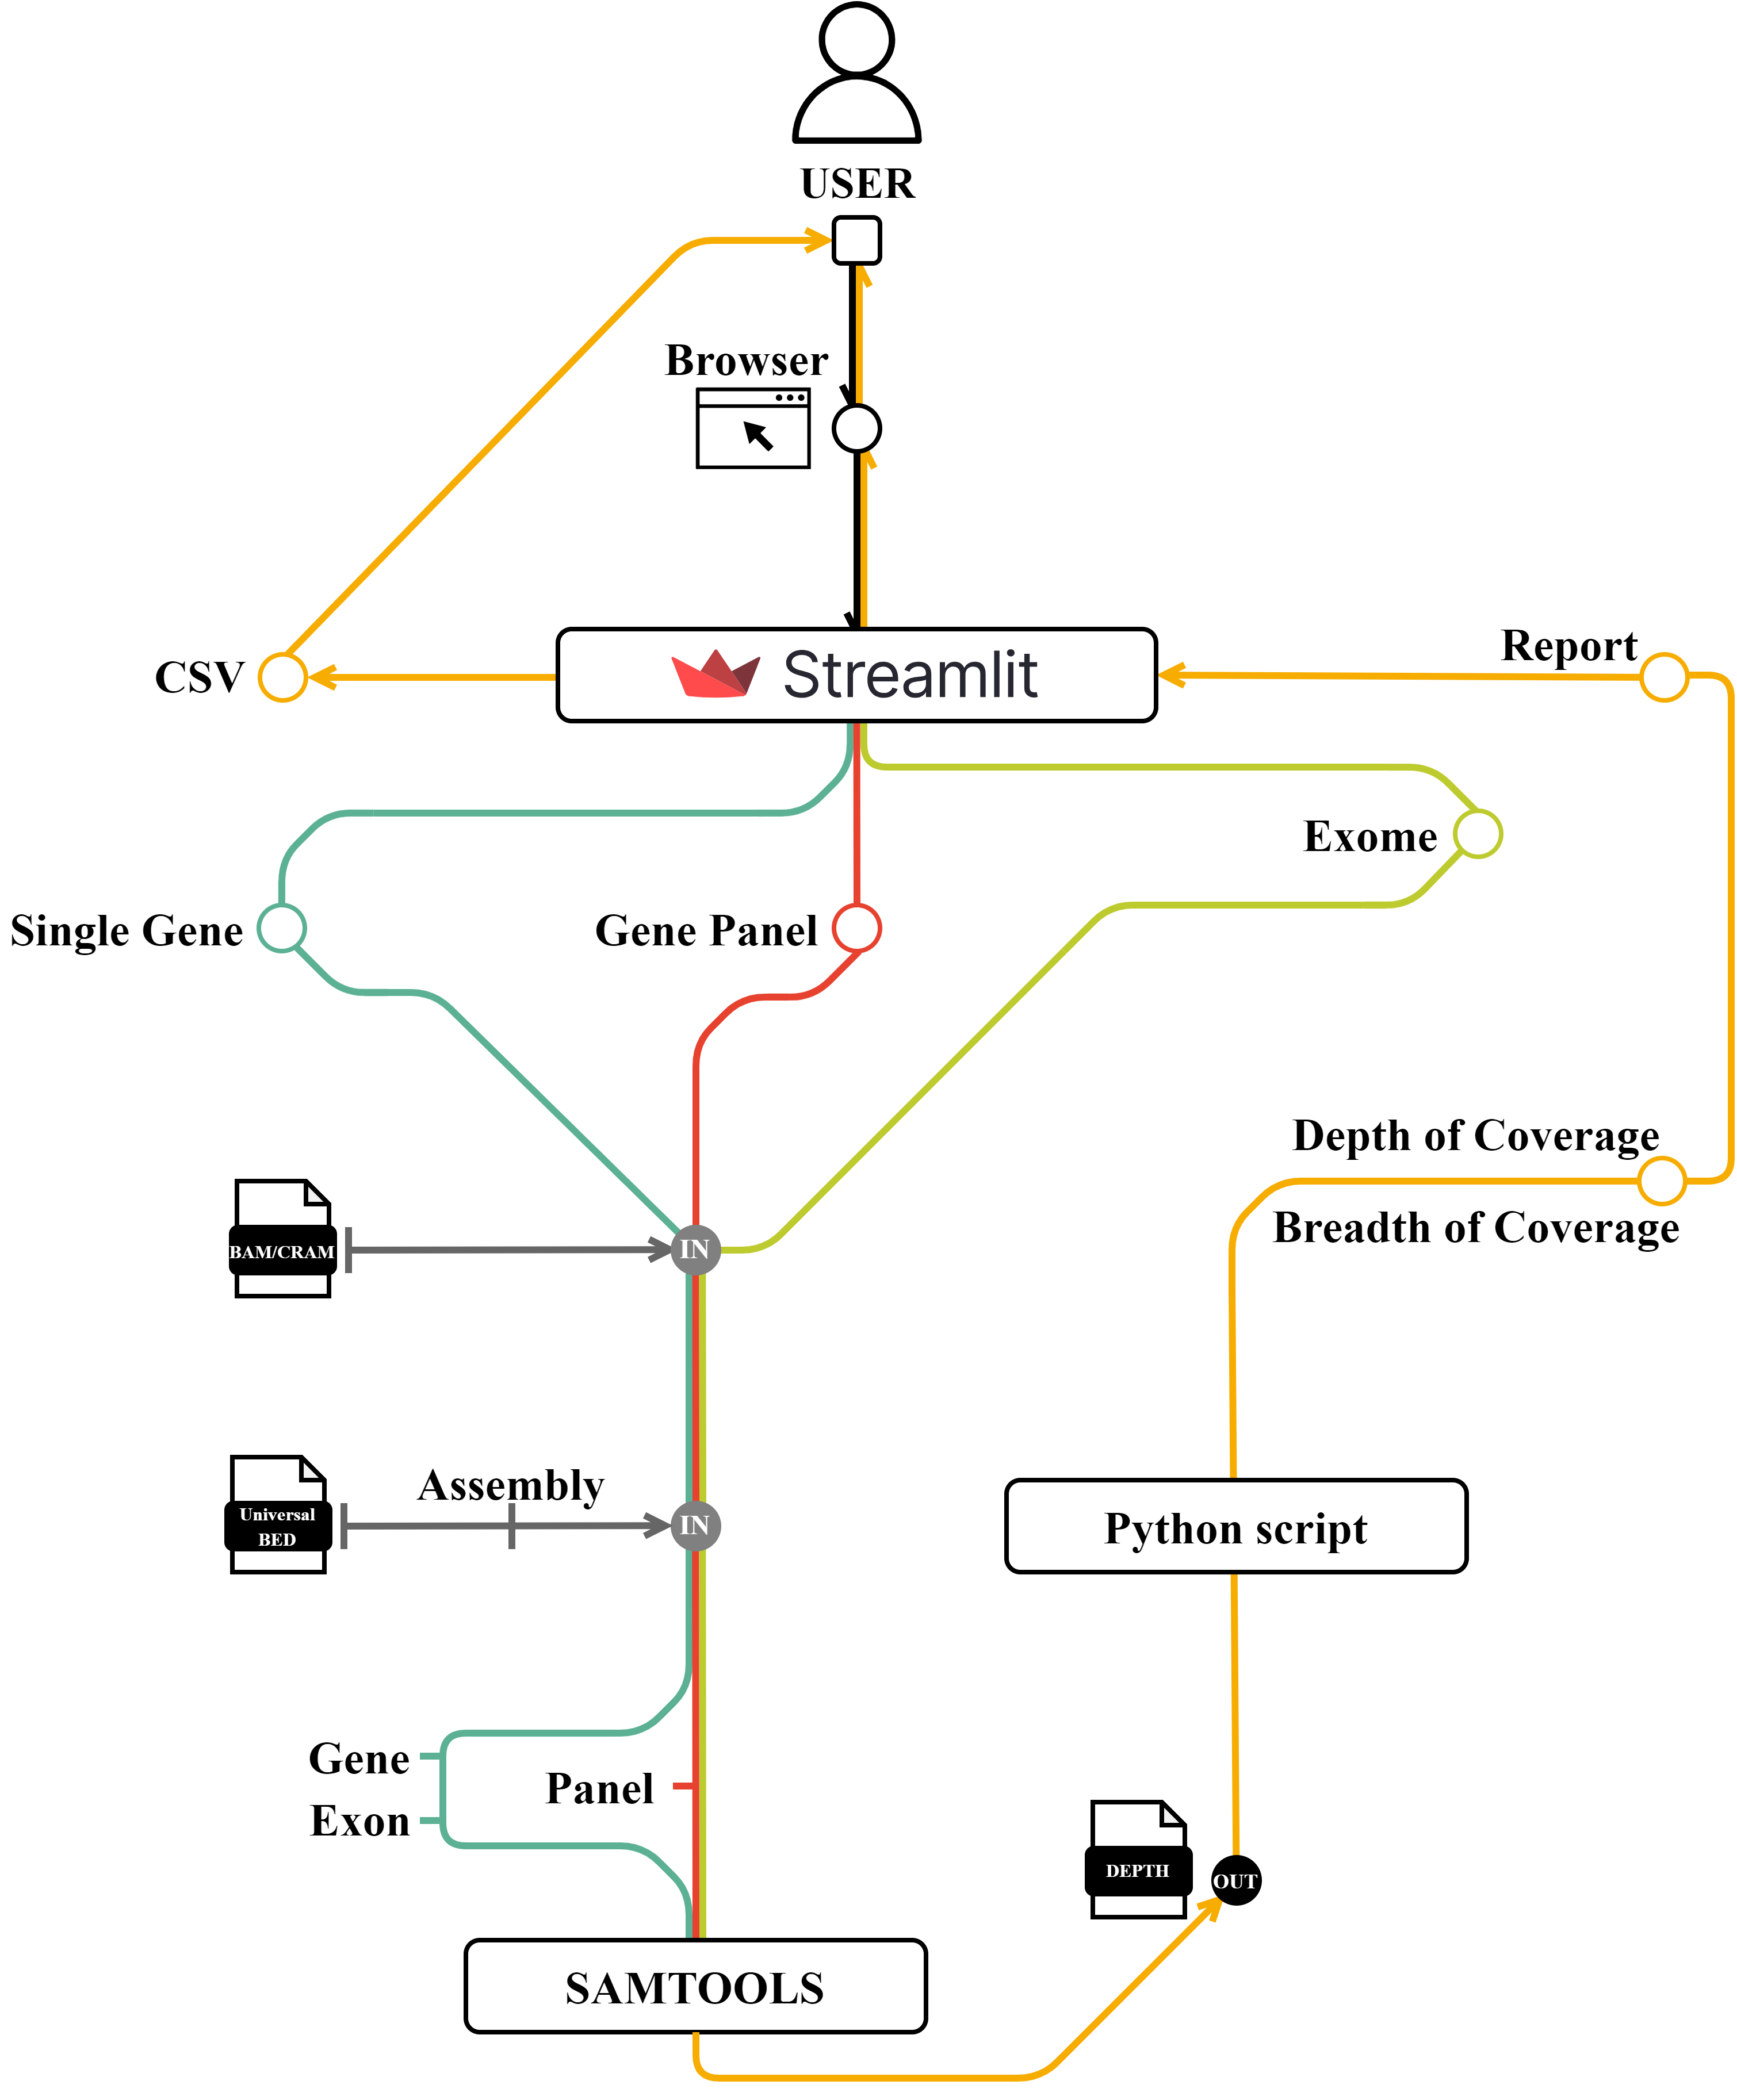
\includegraphics[width=0.7\textwidth]{figs/architecture.png}
    \caption{Scheme of the software architecture.} 
    \label{fig:architecture}
\end{figure}

At the top of the scheme, Streamlit is positioned prominently allowing the user to select what analysis he wants to perform. The Streamlit interface is the central component of the system, symbolizing its role in managing the user interface and orchestrating the pipeline's execution. Streamlit receives input from several sources, including BAM/CRAM files and a Universal \ac{bed} file.

These inputs are fed into a central processing unit, represented by Samtools, a powerful toolkit widely used for manipulating and analyzing high-throughput sequencing data.

From Samtools, a series of processing steps take place. The paths culminate in the generation of a DEPTH output file, which contains Depth of Coverage information for each genomic position analyzed. This DEPTH file is then fed into a Python script for further computation and analysis.

The final output from the Python script is routed back to the Streamlit application, completing the loop. The Streamlit interface is then responsible for displaying the results to the user, allowing them to interact with and visualize the processed data.

The scheme effectively captures the modularity of the system, with Samtools acting as the computational engine, Streamlit as the user interface, and Python handling the data analysis. The diagram highlights the simplicity of the system's architecture while emphasizing the importance of data inputs, the computational process, and the feedback loop to the user interface.

The modularity of the system is demonstrated by the clear separation of components, each with a specific role in the analysis process. The Figure \ref{fig:tree} shows the software directory structure.

\begin{figure}[H]
    \centering
    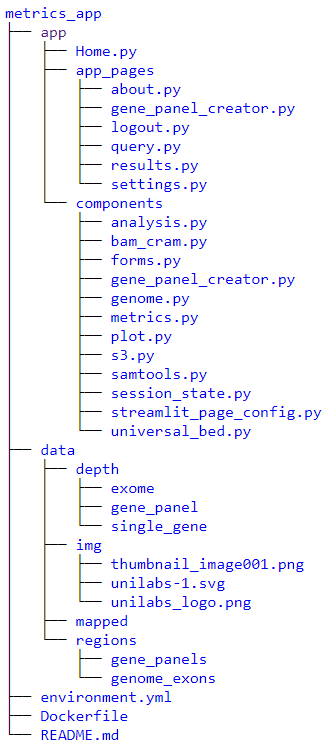
\includegraphics[width=0.3\textwidth]{figs/tree.png}
    \caption{Software directory structure.} 
    \label{fig:tree}
\end{figure}

At the top level, the \texttt{metrics\_app} directory contains core components such as the app logic and necessary resources. The \texttt{app} folder houses the main scripts that drive the application, including \texttt{Home.py}, which serves as the entry point, and submodules like \texttt{app\_pages} for UI-specific components such as \texttt{about.py}, \texttt{query.py}, and \texttt{results.py}. The \texttt{components} directory contains functional modules such as \texttt{analysis.py}, \texttt{metrics.py}, and \texttt{bam\_cram.py}, encapsulating core logic for genome analysis, metrics computation, and file handling. The \texttt{data} folder stores essential files, including genomic depth and region data, which are organized by specific analysis types (e.g., Single Gene, Gene Panel). The project includes setup files like \texttt{environment.yml} for managing dependencies and a \texttt{Dockerfile} to enable containerization for consistent deployment. Overall, the structure supports scalability, modularity, and ease of maintenance. 

\section{Development}

The development of the software followed an iterative and structured approach, with each stage focusing on expanding its functionality while ensuring stability and performance. The process began with the implementation of the Single Gene analysis, which served as the foundation for the project. This initial version was designed to be stable and functional, enabling users to select \ac{bam} or \ac{cram} files and analyze metrics for specific genes with precision.

Once the Single Gene functionality was fully operational, the next phase involved adding support for Gene Panel analysis. This required adjusting the existing framework to handle a broader set of genes while maintaining the same level of accuracy and efficiency. A stable and functional version was again achieved, providing users with the ability to select and analyze predefined gene panels. Each functionality added was versioned using Git and GitHub, ensuring that changes were tracked and managed effectively.

Finally, the software was further enhanced to include Exome analysis, allowing for the comprehensive examination of the entire exome. This functionality was integrated without compromising the stability or performance of the system, and once again, a stable and functional version was built by adding a branch to project's GitHub repository.

Throughout the development, various components and tools were employed to ensure the software met the required performance standards and provided an intuitive user experience. The careful progression from Single Gene to Gene Panel, and finally to Exome analysis, highlights the modularity and scalability of the software, as well as the emphasis placed on testing and validation at each stage.

The following sections provide an overview of the key tools and technologies used in the development of the whole software, including all the stages of the project.

\subsection{Environment preparation}
\subsubsection{\textbf{\acl{wsl}}}

On Windows, developers have access to both the Windows and Linux environments, thanks to the \ac{wsl}. With \ac{wsl}, it is possible to install different Linux distributions, such as Ubuntu, OpenSUSE, Kali, Debian, Arch Linux, among others. This allows Linux applications, utilities and command-line tools to be used directly in Windows, without the need to modify the operating system, resort to virtual machines or dual boot. \cite{wsl}

In the context of the development of this tool, the need to install \ac{wsl} was driven mainly due to the scenario in which many essential tools and software for bioinformatics are designed to work in Linux environments. For this reason, the set of steps recommended on the Microsoft website to configure this environment (Build 19041 or higher) were followed. \cite{wsl}

\subsubsection{\textbf{Anaconda and Conda}}

After installing \ac{wsl}, the installation step of Anaconda (a platform for data science in Python/R that includes conda, a package and environment manager) followed. \cite{anaconda1}

In the case of the creation of the metrics analysis tool, this step was fundamental to allow the installation and maintenance of all the packages and dependencies necessary for the operation of the software. By creating a conda environment, it was possible to ensure that all installed tools work independently without conflicts between versions and packages, thus ensuring the reproducibility of the created software. \cite{anaconda2}

Following the documentation provided by Anaconda, the installation and creation of the conda environment was carried out. \cite{anaconda3} 

Additionally, all the dependencies of the Table \ref{tab:packages} were installed within the created environment. This installation was carried out by installing package by package, however, an environment.yaml file was made available, allowing the bulk installation \cite{anaconda4} of all dependencies on the versions compatible with the software.

\subsubsection{\textbf{Git and GitHub}}

GitHub is a platform that allows users to store, share, and collaborate on code writing with others. \cite{github} Its operation is based on repositories managed by Git, a version control system that tracks all changes made by one or more users in a project. \cite{github} When files are uploaded to GitHub, they become part of the created repository. Any change (commit) to any file is automatically tracked. These changes, made locally, are usually synchronized continuously by pushing the committed changes. Similarly, any changes made locally by another user and synchronized on GitHub can be retrieved by making a pull request. \cite{github}

Thus, by using the documentation of Git and GitHub, this practice was implemented, which not only ensures that each version of the created software is recorded, guaranteeing that the work is not lost and allowing for version rollback in case of bugs, but also ensures that all software produced is reproducible and available for deployment by any user. \cite{github}

\subsection{Streamlit}

The developed software was built using Streamlit which is an open-source Python library designed to enable the swift and intuitive creation of interactive web applications, primarily aimed at data science and machine learning projects. Introduced in October 2019 and now part of the Snowflake ecosystem, Streamlit has quickly gained recognition within the data science community due to its user-friendly approach. Its main goal is to make transforming machine learning scripts into interactive apps as simple as possible, allowing users to incorporate complex features with minimal effort. \cite{Sehm2022}

Streamlit's core philosophy revolves around a declarative, straightforward interface-building model. It enables developers to create apps using clean, concise code without the need for managing intricate state or setting up callbacks, which is common in other frameworks. This makes Streamlit especially suited for rapid prototyping, as well as for displaying machine learning models and data visualizations. The library also seamlessly integrates with many popular Python frameworks for data analysis and visualization. \cite{Sehm2022}

What further sets Streamlit apart is its flexibility and extensibility. The library's architecture allows the integration of various web components, making it easy to customize applications for different use cases. This versatility, along with its growing popularity and adoption in the data science world, has cemented Streamlit as a valuable tool for building interactive, informative applications that can be easily shared and adapted. \cite{Dayanithi2023}

Various Streamlit widgets were used to create the graphical interface of the software, including buttons, text boxes, selectors, among others. Additionally, the library was employed to display the analysis results, also allowing data export to a \ac{csv}/\ac{pdf} file. The integration of Streamlit with Python was crucial in developing an interactive and user-friendly software, meeting the established usability requirements. The functionality and implementation of these widgets are detailed in \cite{streamlit_doc}.

\subsection{Processing and Simplification of \ac{bed} File for Genomic Analysis}

The \ac{bed} files can be highly complex due to its rich annotation. Such complexity is unnecessary for our specific analysis, which focused primarily on gene panel-level, gene-level and exon-level metrics. Therefore, it's essential to simplify \ac{bed} files while preserving relevant genomic data, particularly the coodinates, gene names and exon numbers.

The simplification process involved writing a custom Python script designed to extract and reorganize key elements from the original \ac{bed} file. The script processes each line of the file, extracting the chromosome, start, and end positions, while simplifying the fourth column to retain only the gene name. Additionally, the script distributes exon numbers for each position based on the orientation of the strand.

To facilitate downstream analysis and ensure compatibility with different tools, the script also included an option to remove the "chr" prefix from chromosome identifiers. This was particularly important for certain bioinformatics tools that require the chromosome numbers without this prefix. The option to remove the prefix was controlled by a boolean flag, ensuring flexibility in handling different file formats.

The output of this process was a simplified \ac{bed} file containing six columns: chromosome number, start position, end position, gene name, exon number, and exon length (calculated as the difference between the start and end positions). Below is an example of the resulting file structure:

\begin{verbatim}
    
    (...)
    17	41177976	41178064	RND2	3	88
    17	41179199	41179309	RND2	4	110
    17	41180077	41180212	RND2	5	135
    17	41180448	41180697	RND2	6	249
    17	41181106	41181131	RND2	7	25
    17	41196309	41196310	SNORA40	1	1
    17	41196331	41196332	BRCA1	1	1
    17	41196371	41196372	BRCA1	2	1
    17	41196402	41196403	BRCA1	3	1
    (...)
\end{verbatim}

In this example, the genes spans several lines, each representing a distinct exon. The exon numbers were automatically assigned based on the orientation of the strand, while the genomic intervals for each exon were derived directly from the original \ac{bed} file. The final output, now simplified, facilitates a more straightforward analysis of metrics at both the gene and exon levels. The Python script used for this transformation is outlined in Code \ref{lbl:bed_script}.

\begin{longlisting}
\begin{minted}[
    breaklines,
    breakanywhere,
    bgcolor=LightGray,
    fontsize=\footnotesize,
    linenos
    ]{python}
import argparse

def process_bed_file(input_file, output_file, remove_chr_prefix=False):
    last_gene = None
    exon_count = 0
    
    with open(input_file, 'r') as infile, open(output_file, 'w') as outfile:
        for line in infile:
            fields = line.strip().split('\t')
            
            # Splitting column 4 by the ',' separator
            gene_info = fields[3].split(',')
            gene = gene_info[0]
            
            # Checking if the gene has changed to count exons
            if gene != last_gene:
                exon_count = 1
            else:
                exon_count += 1
            
            # Calculating the difference between $3 and $2
            start = int(fields[1])
            end = int(fields[2])
            diff = end - start
            
            # Remove the "chr" prefix from the chromosome number if needed
            chromosome = fields[0]
            if remove_chr_prefix:
                chromosome = chromosome[3:] if chromosome.startswith("chr") else chromosome
            
            # Updating the last gene
            last_gene = gene
            
            # Writing to the output file
            outfile.write(f"{chromosome}\t{fields[1]}\t{fields[2]}\t{gene}\t{exon_count}\t{diff}\n")

def main():
    parser = argparse.ArgumentParser(description="Process a BED file and optionally remove 'chr' prefix from chromosome numbers.")
    
    parser.add_argument('input_file', help="Path to the input BED file.")
    parser.add_argument('output_file', help="Path to the output BED file.")
    parser.add_argument('--remove-chr-prefix', action='store_true', 
                        help="Remove 'chr' prefix from chromosome names.")

    args = parser.parse_args()
    
    process_bed_file(args.input_file, args.output_file, args.remove_chr_prefix)

if __name__ == "__main__":
    main()
\end{minted}
\caption{Python script for processing and simplifying \ac{bed} files.}
\label{lbl:bed_script}
\end{longlisting}

The script takes an input \ac{bed} file, processes each line, and writes the simplified output to a new file. The script also includes an argument parser to handle command-line options, such as specifying the input and output files and whether to remove the "chr" prefix from chromosome numbers. It can be executed from the command line using a command like \texttt{pyhton universal\_bed.py input.bed output.bed} or with the "--remove-chr-prefix" option enabled. This script was instrumental in preparing the \ac{bed} file for subsequent analysis, ensuring that the data was appropriately formatted and structured for downstream processing.

\subsection{Samtools Depth Calculation in Python with Streamlit}

The \textbf{depth} function from Code \ref{lbl:samtools0} is designed to compute the Depth of Coverage for specific genes and exons from \ac{cram} or \ac{bam} sequencing files. This function integrates Samtools into a Python workflow, allowing users to filter genomic regions dynamically based on the provided genes and exons. By leveraging Streamlit's session state, it retains filtered \ac{bed} content and the depth output for subsequent processing and visualization.

\begin{longlisting}
    \begin{minted}[
        breaklines,
        breakanywhere,
        bgcolor=LightGray,
        fontsize=\footnotesize,
        linenos
        ]{python}
def depth(cram_path, bed_path, depth_dir='data/depth', gene_selection=None, exon_selection=None):
    """
    Calculate the depth of coverage for specific exons of genes in a CRAM/BAM file using samtools.

    Args:
        cram_path (str): Path to the CRAM/BAM file.
        bed_path (str): Path to the Universal BED file containing exon coordinates.
        depth_dir (str, optional): Directory to save the depth output file (optional if storing in session state).
        gene_selection (list or None): List of gene names to include in the depth calculation.
        exon_selection (list or None): List of exon numbers to include in the depth calculation for each gene.

    Returns:
        None
    """
    \end{minted}
    \caption{Python function for calculating Depth of Coverage using Samtools.}
    \label{lbl:samtools0}
    \end{longlisting}

\subsubsection{\textbf{Initial Setup and Session State Initialization}}

The function starts by initializing two important variables within the Streamlit session state: \texttt{depth\_output} and \texttt{filtered\_bed}. These variables will hold, respectively, the Samtools depth output and the filtered \ac{bed} content after processing (Code \ref{lbl:samtools1}). By storing these variables in session state, the function ensures that intermediate results can persist across different user interactions.

\begin{longlisting}
\begin{minted}[
    breaklines,
    breakanywhere,
    bgcolor=LightGray,
    fontsize=\footnotesize,
    linenos
    ]{python}
# Initialize session state attributes if they don't exist
if 'depth_output' not in st.session_state:
    st.session_state.depth_output = {}
    
if 'filtered_bed' not in st.session_state:
    st.session_state.filtered_bed = ""
\end{minted}
\caption{Session state initialization.}
\label{lbl:samtools1}
\end{longlisting}

\subsubsection{\textbf{File Validation and Setup for Gene and Exon Selection}}

Before executing the core logic, the function verifies that the paths provided for the \ac{bam}/\ac{cram} and \ac{bed} files are valid (Code \ref{lbl:samtools2}). This validation ensures that no downstream operations occur with invalid input files, avoiding potential errors during execution. If the provided file paths are incorrect, the function halts, displaying an error message via Streamlit's \texttt{st.error} function.

In cases where specific genes or exons are provided, the function converts these selections into lists, ensuring proper format handling. If no gene or exon selection is provided, the function defaults to reading the original \ac{bed} file and storing its contents in the session state. This setup supports two modes of operation: calculating depth across the entire \ac{bed} file or focusing on specific regions of interest.

\begin{longlisting}
\begin{minted}[
    breaklines,
    breakanywhere,
    bgcolor=LightGray,
    fontsize=\footnotesize,
    linenos
    ]{python}
# Check if paths to the CRAM/BAM and BED files are valid
if not os.path.isfile(cram_path) or not os.path.isfile(bed_path):
    st.error("Invalid file path provided for CRAM/BAM or BED file.")
    return  # Stop execution if the paths are invalid

# Convert gene_selection to a list if it's a string
if isinstance(gene_selection, str):
    gene_selection = [gene_selection]

# Convert exon_selection to a list of strings if it's a list of numbers
if exon_selection is not None:
    exon_selection = list(map(str, exon_selection))  # Convert exon numbers to strings

# If no gene or exon selection is provided, use the original BED file
if gene_selection is None and exon_selection is None:
    try:
        with open(bed_path, 'r') as bed_file:
            st.session_state.filtered_bed = bed_file.read()  # Store original BED content in session state
    except Exception as e:
        st.error(f"Error loading BED file: {e}")
        return  # Stop execution in case of file read error
\end{minted}
\caption{Validation and setup for gene and exon selection.}
\label{lbl:samtools2}
\end{longlisting}

\subsubsection{\textbf{Filtering the \ac{bed} File Based on Gene and Exon Selections}}

When specific genes or exons are provided, the function dynamically filters the \ac{bed} file to isolate only the relevant regions for analysis. This filtering process iterates through the lines of the \ac{bed} file, matching the genes and exons with the user-provided selections. Any lines that match the criteria are retained and stored in the session state (Code \ref{lbl:samtools3}).

This step employs a \texttt{try-except} block to handle potential file processing errors gracefully. If no regions match the provided criteria, an informational message is displayed to the user, and the function exits early. This dynamic filtering enhances the function's flexibility by allowing users to focus on specific genomic intervals, ensuring that only relevant data is processed in subsequent steps.

\begin{longlisting}
\begin{minted}[
    breaklines,
    breakanywhere,
    bgcolor=LightGray,
    fontsize=\footnotesize,
    linenos
    ]{python}
else:
    # Otherwise, filter the BED file based on the gene and exon selection
    filtered_bed_lines = []
    try:
        with open(bed_path, 'r') as bed_file:
            for line in bed_file:
                columns = line.strip().split('\t')

                # Ensure the BED file has at least 6 columns (chr, start, end, gene, exon, size)
                if len(columns) < 6:
                    continue

                chrom, start, end, gene, exon, size = columns[0], columns[1], columns[2], columns[3], columns[4], columns[5]

                # Apply gene filter (multiple genes allowed)
                if gene_selection is None or gene in gene_selection:
                    # Apply exon filter: if exon_selection is None, include all exons for the gene
                    if exon_selection is None or exon in exon_selection:
                        filtered_bed_lines.append(f"{chrom}\t{start}\t{end}\t{gene}\t{exon}\t{size}\n")

        # Check if any filtered BED content was found
        if not filtered_bed_lines:
            st.info("No matching regions found for the provided gene or exon selection.")
            return  # Stop execution if no matching regions found

        # Store filtered BED content in Streamlit session state
        st.session_state.filtered_bed = ''.join(filtered_bed_lines)

    except Exception as e:
        st.error(f"Error filtering BED file: {e}")
        return  # Stop execution in case of file processing error
\end{minted}
\caption{Filtering the \ac{bed} file based on gene and exon selections.}
\label{lbl:samtools3}
\end{longlisting}

\subsubsection{\textbf{Running Samtools and Handling the Depth Output}}

Once the filtered regions are prepared, the function proceeds to run Samtools \texttt{depth} command. This step is also encapsulated in a \texttt{try-except} block to handle potential errors during Samtools execution (Code \ref{lbl:samtools4}). The filtered \ac{bed} content, stored in session state, is passed to Samtools via standard input, allowing the command to compute the Depth of Coverage for the specified regions.

After the Samtools process completes, the function checks whether any depth data was returned. If no data is produced (for example, if no coverage was found in the specified regions), the function exits. If data is present, the depth output is stored in the session state for further use. Optionally, the depth output can also be saved to a file in a specified directory, ensuring that users have access to a persistent output.

\begin{longlisting}
\begin{minted}[
    breaklines,
    breakanywhere,
    bgcolor=LightGray,
    fontsize=\footnotesize,
    linenos
    ]{python}
# Create a unique key for the output based on the CRAM/BAM file name
output_key = os.path.splitext(os.path.basename(cram_path))[0]

# Run samtools depth using the BED content (either original or filtered) from session state
try:
    samtools_command = ['samtools', 'depth', '-b', '-', cram_path]
    samtools_process = subprocess.Popen(samtools_command, stdin=subprocess.PIPE, stdout=subprocess.PIPE, text=True)
    samtools_output, _ = samtools_process.communicate(input=st.session_state.filtered_bed)

    # Check if samtools_output is empty
    if not samtools_output.strip():  # If no output is found
        return  # Stop execution if no data is returned

    # Store samtools output (.depth content) in Streamlit session state as a dictionary
    st.session_state.depth_output[output_key] = samtools_output

    # Optionally, save the depth data to a file
    if depth_dir:
        # Ensure the directory exists
        os.makedirs(depth_dir, exist_ok=True)

        # Define the output depth file path based on the CRAM/BAM file name
        depth_path = os.path.join(depth_dir, f"{output_key}.depth")
        with open(depth_path, 'w') as output_file:
            output_file.write(samtools_output)

except Exception as e:
    st.error(f"Error running samtools depth: {e}")
    return  # Stop execution in case of samtools error
\end{minted}
\caption{Running Samtools and handling depth output.}
\label{lbl:samtools4}
\end{longlisting}

\subsubsection{\textbf{Example Usage of the Depth Function}}

Code \ref{lbl:samtools6} provides an example usage of the \textbf{depth} function. In this scenario, the function is used to compute the depth of coverage for the \textbf{BRCA1} gene across exons 1, 2, and 3 from a given \ac{cram} file. The depth output is stored in a specified directory, ensuring that the results can be accessed for further analysis.

\begin{longlisting}
\begin{minted}[
    breaklines,
    breakanywhere,
    bgcolor=LightGray,
    fontsize=\footnotesize,
    linenos
    ]{python}
depth(
    cram_path="/path/to/sample.cram", 
    bed_path="/path/to/regions.bed", 
    depth_dir="/path/to/output_dir", 
    gene_selection=["BRCA1"], 
    exon_selection=[1, 2, 3]
)
\end{minted}
\caption{Example usage of the depth function.}
\label{lbl:samtools6}
\end{longlisting}

\subsection{Detailed Breakdown of the Python Script for Metrics Calculation}

This section delves into a Python script designed to compute sequencing coverage metrics from DEPTH file outputed by Samtools. The script operates within a Streamlit session, facilitating dynamic filtering of genomic regions and providing statistical summaries for individual genes and exons. Below, it's explored each component of the script in detail, illustrating how it achieves its goal of efficient metrics calculation.

\subsubsection{\textbf{1. Importing Necessary Libraries}}

The script begins by importing essential Python libraries required for data manipulation and interaction with the Streamlit application. The core libraries include \texttt{pandas}, a library that provides robust data structures, such as DataFrames, which facilitate complex data manipulation and analysis, \texttt{io} a module that allows the script to handle in-memory streams, which are particularly useful for reading and processing textual data from files stored in memory and, finally, \texttt{streamlit}, the package who enables the creation of the user interface.

\begin{longlisting}
\begin{minted}[
    breaklines,
    breakanywhere,
    bgcolor=LightGray,
    fontsize=\footnotesize,
    linenos
]{python}
import pandas as pd
import io
import streamlit as st
\end{minted}
\caption{Importing necessary libraries.}
\label{lbl:metrics_import}
\end{longlisting}

\subsubsection{\textbf{2. Defining the Metrics Initialization Function}}

Next, the script defines the \texttt{initialize\_metrics()} function, which is responsible for setting up a consistent data structure for storing various sequencing metrics. This function returns a dictionary where each key corresponds to a specific metric, and all metrics are initialized to zero. This standardization ensures that metrics are consistently tracked and updated throughout the calculation process.

\begin{longlisting}
\begin{minted}[
    breaklines,
    breakanywhere,
    bgcolor=LightGray,
    fontsize=\footnotesize,
    linenos
]{python}
def initialize_metrics():
    return {
        'Size Coding': 0,
        'Size Covered': 0,
        'Breadth of Coverage %': 0,
        'Average Read Depth': 0,
        'Min Read Depth': 0,
        'Max Read Depth': 0,
        'Depth of Coverage % (1x)': 0,
        'Depth of Coverage % (10x)': 0,
        'Depth of Coverage % (15x)': 0,
        'Depth of Coverage % (20x)': 0,
        'Depth of Coverage % (30x)': 0,
        'Depth of Coverage % (50x)': 0,
        'Depth of Coverage % (100x)': 0,
        'Depth of Coverage % (500x)': 0,
        'Depth of Coverage (>500x)': 0,
        'Depth of Coverage (0-1x)': 0,
        'Depth of Coverage (2-10x)': 0,
        'Depth of Coverage (11-15x)': 0,
        'Depth of Coverage (16-20x)': 0,
        'Depth of Coverage (21-30x)': 0,
        'Depth of Coverage (31-50x)': 0,
        'Depth of Coverage (51-100x)': 0,
        'Depth of Coverage (101-500x)': 0
    }
\end{minted}
\caption{Defining the metrics initialization function.}
\label{lbl:metrics_init}
\end{longlisting}

This dictionary structure is critical for the script because it ensures that all necessary metrics, such as Depth of Coverage percentages at various thresholds, are included and consistently tracked. By initializing metrics to zero, the function guarantees that all relevant data fields are present, even if no coverage is detected in certain regions, thereby preventing errors later in the script.

\subsubsection{\textbf{3. Accessing Filtered Data from Session State}}

The \texttt{calculate\_metrics()} function, which handles the core logic of the script, begins by accessing the filtered \ac{bed} content and depth data that were stored in Streamlit's session state during earlier steps. These data sources are crucial for the downstream calculations. If either the \ac{bed} content or the depth data is missing, the function raises a \texttt{ValueError}, ensuring that no further calculations are performed with incomplete or missing data.

\begin{longlisting}
\begin{minted}[
    breaklines,
    breakanywhere,
    bgcolor=LightGray,
    fontsize=\footnotesize,
    linenos
]{python}
def calculate_metrics():
    # Access the filtered BED content and depth data from session_state
    bed_content = st.session_state.get('filtered_bed', '')
    depth_dict = st.session_state.get('depth_output', {})

    if not bed_content:
        raise ValueError("No filtered BED content found in session state.")

    if not depth_dict:
        raise ValueError("No depth data found in session state.")

    results = {}  # Initialize results dictionary
\end{minted}
\caption{Accessing filtered \ac{bed} and depth data from session state.}
\label{lbl:metrics_access}
\end{longlisting}

This step of accessing session state data ensures that the script can efficiently handle user-selected regions of interest (genes and exons or gene panels) and corresponding depth data. This setup also supports interactive workflows where users can refine their selections dynamically, with metrics recalculated based on these selections.

\subsubsection{\textbf{4. Reading the Filtered \ac{bed} Content}}

The filtered \ac{bed} content is then read into a Pandas DataFrame for easier manipulation. This DataFrame contains information about the genomic regions (chromosome, start and end positions, gene names, exon numbers, and exon sizes), which will later be cross-referenced with the depth data to compute metrics.

\begin{longlisting}
\begin{minted}[
    breaklines,
    breakanywhere,
    bgcolor=LightGray,
    fontsize=\footnotesize,
    linenos
]{python}
    # Read the filtered BED content into a DataFrame
    bed_df = pd.read_csv(io.StringIO(bed_content), sep='\t', header=None,
                         names=['CHROM', 'START', 'END', 'GENE', 'EXON', 'SIZE'])
\end{minted}
\caption{Reading filtered \ac{bed} content into a DataFrame.}
\label{lbl:metrics_bed_df}
\end{longlisting}

By converting the \ac{bed} content into a DataFrame, the script leverages Pandas powerful data manipulation capabilities, which streamline tasks such as filtering, grouping, and aggregating genomic regions. This enables efficient computation of metrics for different genes and exons in subsequent steps.

\subsubsection{\textbf{5. Processing Depth Data for Each File}}

Next, the script iterates over each entry in the depth dictionary, where each entry corresponds to a different \ac{bam} or \ac{cram} file. For each file, a new DataFrame is created to hold the depth data, which consists of three columns: chromosome (\texttt{CHROM}), position (\texttt{POS}), and depth (\texttt{DEPTH}).

\begin{longlisting}
\begin{minted}[
    breaklines,
    breakanywhere,
    bgcolor=LightGray,
    fontsize=\footnotesize,
    linenos
]{python}
    for file_name, depth_content in depth_dict.items():
        # Initialize the results structure for this file
        results[file_name] = {}
        
        # Read the depth content into a DataFrame
        depth_df = pd.read_csv(io.StringIO(depth_content), sep='\t', header=None,
                               names=['CHROM', 'POS', 'DEPTH'])
\end{minted}
\caption{Processing depth data for each \ac{bam}/\ac{cram} file.}
\label{lbl:metrics_depth_df}
\end{longlisting}

This iterative approach allows the script to handle multiple samples or files, computing metrics independently for each. This flexibility makes the script suitable for batch processing of sequencing data or for analyzing different samples within the same workflow.

\subsubsection{\textbf{6. Calculating Metrics for All Genes Combined}}

The script then calculates metrics for all genes combined, which provides an overall summary of the metrics across the entire set of regions. Key metrics include the total size of coding regions (\texttt{Size Coding}), the Average Depth of Coverage (\texttt{Average Read Depth}), the Breadth of Coverage.

\begin{longlisting}
\begin{minted}[
    breaklines,
    breakanywhere,
    bgcolor=LightGray,
    fontsize=\footnotesize,
    linenos
]{python}
        # Initialize metrics for all genes
        all_genes_metrics = initialize_metrics()
        total_positions = len(depth_df)

        if total_positions > 0:
            # Extract depth values
            all_depths = depth_df['DEPTH']

            # Calculate Size Coding
            all_genes_metrics['Size Coding'] = bed_df['SIZE'].sum()

            # Calculate Average Read Depth
            all_genes_metrics['Average Read Depth'] = all_depths.mean()
            
            # Calculate Min and Max Read Depth
            all

_genes_metrics['Min Read Depth'] = all_depths.min()
            all_genes_metrics['Max Read Depth'] = all_depths.max()

            # Calculate Size Covered
            all_genes_metrics['Size Covered'] = all_depths.count()

            # Calculate Breadth of Coverage %
            all_genes_metrics['Breadth of Coverage %'] = (
                all_genes_metrics['Size Covered'] / all_genes_metrics['Size Coding']
            ) * 100
\end{minted}
\caption{Calculating metrics for all genes combined.}
\label{lbl:metrics_all_genes}
\end{longlisting}

The calculation of \texttt{Breadth of Coverage \%} is particularly important for assessing the quality of sequencing coverage, as it indicates the proportion of the target regions that have been successfully sequenced. These metrics provide a high-level overview of the data, serving as a starting point for more granular analysis at the gene and exon levels.

\subsubsection{\textbf{7. Calculating Depth of Coverage Percentages}}

For each depth threshold (e.g., 1x, 10x, 15x, etc.), the script computes the percentage of positions that meet or exceed that depth. These depth thresholds are commonly used in sequencing to assess the reliability of variant calls or to ensure sufficient coverage for accurate analysis.

\begin{longlisting}
\begin{minted}[
    breaklines,
    breakanywhere,
    bgcolor=LightGray,
    fontsize=\footnotesize,
    linenos
]{python}
            # Define coverage thresholds
            coverage_thresholds = [1, 10, 15, 20, 30, 50, 100, 500]

            # Calculate counts for each threshold
            coverage_counts = {
                threshold: (all_depths >= threshold).sum() for threshold in coverage_thresholds
            }

            # Calculate percentages
            for threshold in coverage_thresholds:
                all_genes_metrics[f"Depth of Coverage % ({threshold}x)"] = (
                    coverage_counts[threshold] / total_positions
                ) * 100
\end{minted}
\caption{Calculating depth of coverage percentages for different thresholds.}
\label{lbl:metrics_coverage}
\end{longlisting}

By calculating these percentages, the script provides insight into how well each region is covered at different depths, helping to identify any coverage gaps that might impact downstream analysis. These metrics are critical for quality control and for determining whether additional sequencing is needed.

\subsubsection{\textbf{8. Calculating Depth Intervals}}

In addition to calculating Depth of Coverage percentages for fixed thresholds, the script also computes the number of positions that fall within specific depth intervals. This helps to understand the distribution of Depth of Coverage across the different thresholds.

\begin{longlisting}
\begin{minted}[
    breaklines,
    breakanywhere,
    bgcolor=LightGray,
    fontsize=\footnotesize,
    linenos
]{python}
            # Define depth intervals and calculate counts
            depth_intervals = {
                "Depth of Coverage (>500x)": (all_depths > 500).sum(),
                "Depth of Coverage (101-500x)": ((all_depths > 100) & (all_depths <= 500)).sum(),
                "Depth of Coverage (51-100x)": ((all_depths >= 51) & (all_depths <= 100)).sum(),
                "Depth of Coverage (31-50x)": ((all_depths >= 31) & (all_depths <= 50)).sum(),
                "Depth of Coverage (21-30x)": ((all_depths >= 21) & (all_depths <= 30)).sum(),
                "Depth of Coverage (16-20x)": ((all_depths >= 16) & (all_depths <= 20)).sum(),
                "Depth of Coverage (11-15x)": ((all_depths >= 11) & (all_depths <= 15)).sum(),
                "Depth of Coverage (2-10x)": ((all_depths >= 2) & (all_depths <= 10)).sum(),
                "Depth of Coverage (0-1x)": (all_depths <= 1).sum(),
            }

            # Update the metrics dictionary
            all_genes_metrics.update(depth_intervals)
\end{minted}
\caption{Calculating counts for specific depth intervals.}
\label{lbl:metrics_intervals}
\end{longlisting}

\subsubsection{\textbf{9. Calculating Metrics for Each Gene}}

The script proceeds to calculate individual metrics for each gene. It filters the \ac{bed} DataFrame to extract the corresponding regions, and then accumulates depth values across all positions in those regions. Metrics such as Average Read Depth, Minimum and Maximum Read Depth are calculated for each gene.

\begin{longlisting}
\begin{minted}[
    breaklines,
    breakanywhere,
    bgcolor=LightGray,
    fontsize=\footnotesize,
    linenos
]{python}
            # Initialize dictionaries to hold gene and exon metrics
            genes_data = {}
            exons_data = {}
            genes = bed_df['GENE'].unique()

            for gene in genes:
                # Initialize metrics for the gene
                gene_metrics = initialize_metrics()
                gene_bed_df = bed_df[bed_df['GENE'] == gene]

                # Calculate Size Coding for the gene
                gene_metrics['Size Coding'] = gene_bed_df['SIZE'].sum()

                # Initialize a Series to hold depth values for the gene
                gene_depths = pd.Series(dtype=float)

                # Accumulate depth values for all exons in the gene
                for _, row in gene_bed_df.iterrows():
                    start = row['START']
                    end = row['END']
                    exon_depths = depth_df[
                        (depth_df['POS'] >= start) & (depth_df['POS'] <= end)
                    ]['DEPTH']
                    gene_depths = pd.concat([gene_depths, exon_depths], ignore_index=True)

                if len(gene_depths) > 0:
                    # Calculate metrics for the gene
                    gene_metrics['Average Read Depth'] = gene_depths.mean()
                    gene_metrics['Min Read Depth'] = gene_depths.min()
                    gene_metrics['Max Read Depth'] = gene_depths.max()
                    gene_metrics['Size Covered'] = gene_depths.count()
                    gene_metrics['Breadth of Coverage %'] = (
                        gene_metrics['Size Covered'] / gene_metrics['Size Coding']
                    ) * 100
                else:
                    # Set metrics to zero if no depth data is available
                    gene_metrics['Average Read Depth'] = 0
                    gene_metrics['Min Read Depth'] = 0
                    gene_metrics['Max Read Depth'] = 0
                    gene_metrics['Size Covered'] = 0
\end{minted}
\caption{Calculating metrics for each gene.}
\label{lbl:metrics_gene}
\end{longlisting}

This gene-specific analysis allows the script to provide detailed metrics that are relevant for studying individual genes. These metrics can be used to assess whether particular genes have been sequenced sufficiently for downstream analyses, such as variant calling or expression analysis.

\subsubsection{\textbf{10. Calculating Depth of Coverage Percentages for Each Gene}}

As with the overall analysis, the script calculates also Depth of Coverage percentages for each gene at various thresholds. This ensures that the analysis can identify specific genes that may have insufficient coverage for reliable variant calling or other analyses.

\begin{longlisting}
\begin{minted}[
    breaklines,
    breakanywhere,
    bgcolor=LightGray,
    fontsize=\footnotesize,
    linenos
]{python}
                # Calculate coverage percentages for the gene
                coverage_counts_gene = {
                    threshold: (gene_depths >= threshold).sum() for threshold in coverage_thresholds
                }

                for threshold in coverage_thresholds:
                    gene_metrics[f"Depth of Coverage % ({threshold}x)"] = (
                        coverage_counts_gene[threshold] / gene_metrics['Size Covered']
                    ) * 100 if gene_metrics['Size Covered'] > 0 else 0

                # Calculate depth intervals for the gene
                depth_intervals_gene = {
                    "Depth of Coverage (>500x)": (gene_depths > 500).sum(),
                    "Depth of Coverage (101-500x)": ((gene_depths > 100) & (gene_depths <= 500)).sum(),
                    # ... (other intervals)
                }

                gene_metrics.update(depth_intervals_gene)

                # Store the gene metrics
                genes_data[gene] = gene_metrics
\end{minted}
\caption{Calculating depth percentages and intervals for each gene.}
\label{lbl:metrics_gene_coverage}
\end{longlisting}


\subsubsection{\textbf{11. Calculating Metrics for Each Exon Within Each Gene}}

The script also calculates metrics for individual exons within each gene. By breaking down the analysis to the exon level, the script provides a finer level of detail that can be useful for studying specific exonic regions, especially in clinical or functional genomics applications.

\begin{longlisting}
\begin{minted}[
    breaklines,
    breakanywhere,
    bgcolor=LightGray,
    fontsize=\footnotesize,
    linenos
]{python}
                # Initialize a dictionary to hold exon metrics for the gene
                exon_data_for_gene = {}
                
                for exon_name in gene_bed_df['EXON'].unique():
                    # Initialize metrics for the exon
                    exon_metrics = initialize_metrics()
                    exon_bed_df = gene_bed_df[gene_bed_df['EXON'] == exon_name]
                    exon_depths = pd.Series(dtype=float)
                    
                    exon_metrics['Size Coding'] = exon_bed_df['SIZE'].sum()

                    for _, row in exon_bed_df.iterrows():
                        start = row['START']
                        end = row['END']
                        exon_depths = pd.concat([
                            exon_depths,
                            depth_df[(depth_df['POS'] >= start) & (depth_df['POS'] <= end)]['DEPTH']
                        ], ignore_index=True)

                    if len(exon_depths) > 0:
                        # Calculate metrics for the exon
                        exon_metrics['Average Read Depth'] = exon_depths.mean()
                        exon_metrics['Min Read Depth'] = exon_depths.min()
                        exon_metrics['Max Read Depth'] = exon_depths.max()
                        exon_metrics['Size Covered'] = exon_depths.count()
                        exon_metrics['Breadth of Coverage %'] = (
                            exon_metrics['Size Covered'] / exon_metrics['Size Coding']
                        ) * 100
                    else:
                        # Set metrics to zero if no depth data is available
                        exon_metrics['Average Read Depth'] = 0
                        exon_metrics['Min Read Depth'] = 0
                        exon_metrics['Max Read Depth'] = 0
                        exon_metrics['Size Covered'] = 0

                    # Calculate coverage percentages and intervals for the exon
                    coverage_counts_exon = {
                        threshold: (exon_depths >= threshold).sum() for threshold in coverage_thresholds
                    }

                    for threshold in coverage_thresholds:
                        exon_metrics[f"Depth of Coverage % ({threshold}x)"] = (
                            coverage_counts_exon[threshold] / exon_metrics['Size Covered']
                        ) * 100 if exon_metrics['Size Covered'] > 0 else 0

                    depth_intervals_exon = {
                        "Depth of Coverage (>500x)": (exon_depths > 500).sum(),
                        # ... (other intervals)
                    }

                    exon_metrics.update(depth_intervals_exon)

                    # Store the exon metrics under the gene
                    exon_data_for_gene[exon_name] = exon_metrics

                # Store all exon metrics for the gene
                exons_data[gene] = exon_data_for_gene
\end{minted}
\caption{Calculating metrics for each exon within each gene.}
\label{lbl:metrics_exon}
\end{longlisting}

This level of analysis is especially useful for pinpointing specific exons that may have insufficient coverage for accurate variant detection or expression analysis, which is critical in clinical settings where exonic variants can be associated with disease.

\subsubsection{\textbf{12. Compiling Final Results}}

Finally, the script compiles all the calculated metrics into a comprehensive results structure. This structure contains metrics for the entire set of genes combined (only if the analyses is Gene Panel), as well as per-gene and per-exon metrics. These results can then be used for visualization, reporting, or further analysis.

\begin{longlisting}
\begin{minted}[
    breaklines,
    breakanywhere,
    bgcolor=LightGray,
    fontsize=\footnotesize,
    linenos
]{python}
            # Store the overall metrics, gene metrics, and exon metrics in the results
            results[file_name]['All Genes'] = all_genes_metrics
            results[file_name]['Genes'] = genes_data
            results[file_name]['Exons'] = exons_data

    return results
\end{minted}
\caption{Storing and returning the calculated metrics.}
\label{lbl:metrics_results}
\end{longlisting}

\subsubsection{\textbf{13. Error Handling and Edge Cases}}

Throughout the script, careful attention is given to error handling and edge cases to ensure robustness. For example, the script checks for missing or incomplete data in the session state, handles division by zero errors when calculating percentages, and sets zero as default value in the Dataframe when no Depth of Coverage data is available for a particular gene or exon.

\subsection{Results Generation and Display Functionality}

This section explains the \texttt{results.py} script, which is responsible for generating and displaying sequencing metrics using Streamlit. The script processes metrics data, organizes the results into tables, generates a plot, provides functionality to download a \ac{pdf} report, and dynamically handles multiple samples. It allows users to interactively select and filter metrics, enhancing the flexibility and user-friendliness of the genomic data analysis workflow.

\subsubsection{\textbf{Importing Necessary Libraries and Displaying Logos}}

The script begins by importing the necessary libraries and modules required for its operation (Code \ref{code:results-imports}). It imports standard libraries such as \texttt{pandas} for data manipulation, \texttt{numpy} for numerical operations, and \texttt{datetime} for handling date and time. It also imports custom components from the \texttt{components}, which includes \texttt{metrics}, \texttt{plot}, and \texttt{session\_state} modules. Additionally, it imports \texttt{io} for input\/output operations and \texttt{weasyprint} for generating \ac{pdf} reports. The \texttt{base64} module is used for encoding images for embedding in the \ac{pdf}.

\begin{longlisting}
\begin{minted}[
    breaklines,
    breakanywhere,
    bgcolor=LightGray,
    fontsize=\footnotesize,
    linenos
]{python}
import streamlit as st
import pandas as pd
from components import metrics, plot, session_state
import numpy as np
import io
from weasyprint import HTML
import base64
import datetime
\end{minted}
\caption{Importing necessary libraries and modules for the script.}
\label{code:results-imports}
\end{longlisting}

Next, the script defines the file paths for the sidebar and main body logos (Code \ref{code:results-logos}). These images are used to enhance the visual appeal of the application. The \texttt{st.logo()} function is utilized to display the logos within the Streamlit application. The \texttt{sidebar\_logo} is displayed in the sidebar, while the \texttt{main\_body\_logo} serves as the icon image.

\begin{longlisting}
\begin{minted}[
    breaklines,
    breakanywhere,
    bgcolor=LightGray,
    fontsize=\footnotesize,
    linenos
]{python}
sidebar_logo = "data/img/unilabs_logo.png"
main_body_logo = "data/img/thumbnail_image001.png"
st.logo(sidebar_logo, icon_image=main_body_logo)

st.title("Results")
\end{minted}
\caption{Defining logo file paths and displaying them in the application.}
\label{code:results-logos}
\end{longlisting}

\subsubsection{\textbf{Defining Metric Filters and Helper Functions}}

The script defines helper functions to facilitate the interactive selection and filtering of metrics displayed to the user. The \texttt{render\_metric\_filters} function is responsible for rendering the metric filters within a popover UI element (Code \ref{code:results-render-metric-filters}). It uses Streamlit's \texttt{st.popover} to create a popover window where users can select which metrics to display.

\begin{longlisting}
\begin{minted}[
    breaklines,
    breakanywhere,
    bgcolor=LightGray,
    fontsize=\footnotesize,
    linenos
]{python}
@st.fragment
def render_metric_filters(tab_name, metrics_dict):
    with st.popover("Filters"):
        st.subheader("Select Metrics to Display")

        # Verifies if all metrics are selected
        all_selected = all(
            st.session_state.get(f"{tab_name}_metric_{metric}", False)
            for metrics_list in metrics_dict.values()
            for metric in metrics_list
        )

        # Button to select/deselect all metrics
        if st.button("Select All" if not all_selected else "Deselect All", key=f"{tab_name}_select_all"):
            select_all_metrics(not all_selected, metrics_dict, tab_name)
            st.rerun()

        # Divide the UI into 3 columns
        col1, col2, col3 = st.columns(3)
        metrics_keys = list(metrics_dict.keys())

        # Display the metrics within the columns
        for i, section in enumerate(metrics_keys):
            with [col1, col2, col3][i % 3]:
                st.write(f"**{section}**")
                for metric in metrics_dict[section]:
                    st.checkbox(metric, key=f"{tab_name}_metric_{metric}")
\end{minted}
\caption{Defining the `render\_metric\_filters` function for metric selection.}
\label{code:results-render-metric-filters}
\end{longlisting}

This function first checks if all metrics are selected by iterating over the metrics in \texttt{metrics\_dict} and checking their corresponding values in \texttt{st.session\_state}. It then provides a button to select or deselect all metrics. The metrics are displayed in three columns for better readability, and each metric is represented as a checkbox.

Another helper function, \texttt{select\_all\_metrics}, is defined to handle the selection or deselection of all metrics (Code \ref{code:results-select-all-metrics}). This function updates the \texttt{st.session\_state} for each metric to reflect the user's choice.

\begin{longlisting}
\begin{minted}[
    breaklines,
    breakanywhere,
    bgcolor=LightGray,
    fontsize=\footnotesize,
    linenos
]{python}
def select_all_metrics(select_all, metrics_dict, key_prefix):
    """Function to select or deselect all metrics."""
    for section, metrics_list in metrics_dict.items():
        for metric in metrics_list:
            st.session_state[f"{key_prefix}_metric_{metric}"] = select_all
\end{minted}
\caption{Defining the `select\_all\_metrics` function to toggle metric selection.}
\label{code:results-select-all-metrics}
\end{longlisting}

\subsubsection{\textbf{Defining the Desired Metrics Order}}

To ensure consistency in the presentation of metrics across different DataFrames, the script defines a list \texttt{desired\_order} that specifies the order in which metrics should appear (Code \ref{code:results-desired-order}).

\begin{longlisting}
\begin{minted}[
    breaklines,
    breakanywhere,
    bgcolor=LightGray,
    fontsize=\footnotesize,
    linenos
]{python}
# Desired order of metrics
desired_order = [
    'Size Coding', 'Size Covered', 'Breadth of Coverage %', 'Average Read Depth', 'Min Read Depth', 'Max Read Depth',
    'Depth of Coverage (0-1x)', 'Depth of Coverage (2-10x)', 'Depth of Coverage (11-15x)', 'Depth of Coverage (16-20x)',
    'Depth of Coverage (21-30x)', 'Depth of Coverage (31-50x)', 'Depth of Coverage (51-100x)',
    'Depth of Coverage (101-500x)', 'Depth of Coverage (>500x)',
    'Depth of Coverage % (1x)', 'Depth of Coverage % (10x)', 'Depth of Coverage % (15x)', 'Depth of Coverage % (20x)',
    'Depth of Coverage % (30x)', 'Depth of Coverage % (50x)', 'Depth of Coverage % (100x)', 'Depth of Coverage % (500x)'
]
\end{minted}
\caption{Defining the desired metrics order for display.}
\label{code:results-desired-order}
\end{longlisting}

This ordered list was used later in the script when constructing DataFrames to display metrics in the specified sequence.

\subsubsection{\textbf{Calculating Metrics and Preparing DataFrames}}

The script calls the \texttt{calculate\_metrics()} function from the \texttt{metrics} module to compute sequencing coverage metrics for one or multiple samples (Code \ref{code:results-calculate-metrics}). The results are stored in a dictionary, where each key corresponds to a sample file name, and the value is another dictionary containing metrics for that sample.

\begin{longlisting}
\begin{minted}[
    breaklines,
    breakanywhere,
    bgcolor=LightGray,
    fontsize=\footnotesize,
    linenos
]{python}
# Call the calculate_metrics function and store results for multiple depth files
results = metrics.calculate_metrics()
file_names = list(results.keys())
\end{minted}
\caption{Calculating metrics and obtaining results for samples.}
\label{code:results-calculate-metrics}
\end{longlisting}

To display metrics for all combined genes, the script constructs the DataFrame \texttt{all\_genes\_df} (Code \ref{code:results-all-genes-df}). It starts by creating a list \texttt{all\_metrics} that aligns with the desired order of metrics. Then, the script initializes the DataFrame with a 'Metric' column populated by the metrics from \texttt{all\_metrics}. For each sample, it retrieves the respective metrics from the \texttt{results} dictionary and adds them as new columns in the DataFrame, associating each sample's metrics to the corresponding file key.

\begin{longlisting}
\begin{minted}[
    breaklines,
    breakanywhere,
    bgcolor=LightGray,
    fontsize=\footnotesize,
    linenos
]{python}
# Prepare All Genes DataFrame
all_metrics = desired_order
all_genes_df = pd.DataFrame({'Metric': all_metrics})

for file_key in results:
    all_genes_metrics = results[file_key].get('All Genes', {})
    metrics_values = [all_genes_metrics.get(metric, np.nan) for metric in all_metrics]
    all_genes_df[file_key] = metrics_values
\end{minted}
\caption{Preparing the DataFrame for all genes metrics.}
\label{code:results-all-genes-df}
\end{longlisting}

For gene-level metrics, the script compiles a set of all genes present in the results and creates individual DataFrames for each gene (Code \ref{code:results-genes-dfs}). It iterates over the list of genes, initializes a DataFrame for each, and populates it with metrics from each sample.

\begin{longlisting}
\begin{minted}[
    breaklines,
    breakanywhere,
    bgcolor=LightGray,
    fontsize=\footnotesize,
    linenos
]{python}
# Prepare Genes DataFrames
all_genes_set = set()
for file_key in results:
    genes = results[file_key].get('Genes', {}).keys()
    all_genes_set.update(genes)
genes_list = sorted(all_genes_set)

genes_dfs = {}
for gene in genes_list:
    gene_metrics_df = pd.DataFrame({'Metric': desired_order})
    for file_key in results:
        gene_metrics = results[file_key].get('Genes', {}).get(gene, {})
        metrics_values = [gene_metrics.get(metric, np.nan) for metric in desired_order]
        gene_metrics_df[file_key] = metrics_values
    genes_dfs[gene] = gene_metrics_df
\end{minted}
\caption{Preparing individual DataFrames for each gene.}
\label{code:results-genes-dfs}
\end{longlisting}

Similarly, for exon-level metrics, the script prepares DataFrames for each exon within each gene (Code \ref{code:results-exons-dfs}). It constructs a nested dictionary \texttt{exons\_dfs}, where the keys are gene names, and the values are dictionaries of exon DataFrames.

\begin{longlisting}
\begin{minted}[
    breaklines,
    breakanywhere,
    bgcolor=LightGray,
    fontsize=\footnotesize,
    linenos
]{python}
# Prepare Exons DataFrames
exons_dfs = {}
for gene in genes_list:
    exons_dfs[gene] = {}
    exons_set = set()
    for file_key in results:
        exons = results[file_key].get('Exons', {}).get(gene, {}).keys()
        exons_set.update(exons)
    exons_list = sorted(exons_set)

    for exon in exons_list:
        exon_metrics_df = pd.DataFrame({'Metric': desired_order})
        for file_key in results:
            exon_metrics = results[file_key].get('Exons', {}).get(gene, {}).get(exon, {})
            metrics_values = [exon_metrics.get(metric, np.nan) for metric in desired_order]
            exon_metrics_df[file_key] = metrics_values
        exons_dfs[gene][exon] = exon_metrics_df
\end{minted}
\caption{Preparing DataFrames for exon-level metrics.}
\label{code:results-exons-dfs}
\end{longlisting}

These DataFrames are used later to display metrics in the application and generate reports.

\subsubsection{\textbf{Generating and Downloading the \ac{pdf} Report}}

The script includes functionality to generate a \ac{pdf} report of the metrics for a selected sample. It uses WeasyPrint to convert HTML content into a \ac{pdf}. The report includes the Unilabs logo, the report generation date, and the metrics tables for the selected sample (Code \ref{code:results-generate-report}).

\begin{longlisting}
\begin{minted}[
    breaklines,
    breakanywhere,
    bgcolor=LightGray,
    fontsize=\footnotesize,
    linenos
]{python}
# Download Report section
with st.status("Building the report...")as status:
    if len(file_names) > 1:
        # If there are multiple samples, allow the user to select one
        selected_sample = st.selectbox("Select Sample", file_names)
    else:
        # If there's only one sample, select it by default
        selected_sample = file_names[0]
        
        st.write(f'Download {selected_sample} report file (.pdf)')
    # Generate PDF report for the selected sample
    # Get the current date and time
    report_date = datetime.datetime.now().strftime("%Y-%m-%d %H:%M:%S")
    
    # Build an HTML string
    html_content = """
    <html>
    <head>
    <style>
    body {
        font-family: Arial, sans-serif;
    }
    table {
        border-collapse: collapse;
        width: 100%;
        font-size: 10pt;
    }
    th, td {
        text-align: left;
        padding: 8px;
        border: 1px solid #dddddd;
    }
    tr:nth-child(even) {
        background-color: #f9f9f9;
    }
    h2, h3 {
        color: #2F5496;
    }
    </style>
    </head>
    <body>
    """
    # Add Unilabs logo
    # Encode the logo image to base64
    with open(sidebar_logo, "rb") as image_file:
        encoded_string = base64.b64encode(image_file.read()).decode()
    html_content += f'<img src="data:image/png;base64,{encoded_string}" alt="Unilabs Logo" style="width:200px;"><br><br>'
    # Add report generation date
    html_content += f'<p>Report generated on: {report_date}</p>'
    # Add Overview DataFrame for the selected sample
    html_content += f'<h2>Overview - Sample: {selected_sample}</h2>'
    if st.session_state.analysis in ['Gene Panel']:
        html_content += f'<p>Gene Panel: {st.session_state.panel_name}</p>'
        overview_df = all_genes_df[['Metric', selected_sample]]
        html_content += overview_df.to_html(index=False)
    if st.session_state.analysis in ['Exome']:
        html_content += f'<p>Exome</p>'
        overview_df = all_genes_df[['Metric', selected_sample]]
        html_content += overview_df.to_html(index=False)
    elif st.session_state.analysis in ['Single Gene']:
        # Add Gene DataFrames for the selected sample
        for gene_name, gene_df in genes_dfs.items():
            gene_sample_df = gene_df[['Metric', selected_sample]]
            if gene_sample_df[selected_sample].notna().any():
                html_content += f'<h2>Gene: {gene_name}</h2>'
                html_content += gene_sample_df.to_html(index=False)
        # Add Exon DataFrames for the selected sample
        for gene_name, exons_dict in exons_dfs.items():
            for exon_name, exon_df in exons_dict.items():
                exon_sample_df = exon_df[['Metric', selected_sample]]
                if exon_sample_df[selected_sample].notna().any():
                    html_content += f'<h3>Exon: {exon_name} (Gene: {gene_name})</h3>'
                    html_content += exon_sample_df.to_html(index=False)
    html_content += '</body></html>'
    # Convert HTML to PDF using WeasyPrint
    html_obj = HTML(string=html_content)
    pdf_bytes = html_obj.write_pdf()
    status.update(label="Generating PDF...")
    # Provide download button
    st.download_button(
        label="Download",
        data=pdf_bytes,
        file_name=f'report_{selected_sample}.pdf',
        mime='application/pdf'
    )
    status.update(label="Report ready for download", expanded=True)
\end{minted}
\caption{Generating and downloading a \ac{pdf} report for the selected sample.}
\label{code:results-generate-report}
\end{longlisting}

In this code, the script checks the number of samples and allows the user to select one if multiple samples are present. It then builds an HTML string that includes styling, the logo, the report date, and the metrics tables. The HTML content is converted to a \ac{pdf}, and a download button is provided for the user to save the report.

\subsubsection{\textbf{Creating Tabs Based on Analysis Type}}

The script determines which tabs to display based on the type of analysis stored in \texttt{st.session\_state.analysis} (Code \ref{code:results-create-tabs}). It supports analysis types such as "Gene Panel", "Single Gene", and "Exome". Depending on the analysis type, it creates appropriate tabs like "Overview", "Gene Detail", and "Exon Detail".

\begin{longlisting}
\begin{minted}[
    breaklines,
    breakanywhere,
    bgcolor=LightGray,
    fontsize=\footnotesize,
    linenos
]{python}
# Determine which tabs to display based on st.session_state.analysis
if st.session_state.analysis == 'Gene Panel':
    tab_names = ["Overview", "Gene Detail", "Exon Detail"]
elif st.session_state.analysis in ['Single Gene', 'Exome']:
    tab_names = ["Gene Detail", "Exon Detail"]
else:
    st.warning("Unsupported analysis type.")
    tab_names = []

# Create the tabs
tabs = st.tabs(tab_names)

# Map tab names to tab objects for easy reference
tab_dict = dict(zip(tab_names, tabs))
\end{minted}
\caption{Creating tabs based on the type of analysis.}
\label{code:results-create-tabs}
\end{longlisting}

This dynamic tab creation ensures that the application displays relevant information based on the user's analysis context.

\subsubsection{\textbf{Displaying Metrics in the "Overview" Tab}}

In the "Overview" tab, the script displays general information such as the report date, the analyzed files, and the gene panel name (Code \ref{code:results-overview-tab}). It uses the \texttt{render\_metric\_filters} function to allow users to select which metrics to display and the DataFrame is then displayed using \texttt{st.dataframe}.

\begin{longlisting}
\begin{minted}[
    breaklines,
    breakanywhere,
    bgcolor=LightGray,
    fontsize=\footnotesize,
    linenos
]{python}
if "Overview" in tab_dict:
    with tab_dict["Overview"]:
        st.write(f"Date: {report_date}")
        st.write(f"Analyzing file(s): {file_names}")
        st.write(f"Gene Panel: {st.session_state.panel_name}")

        if st.session_state.analysis in ['Gene Panel', 'Exome']:
            
            with st.container():
                # Use 'metrics_dict' instead of 'columns' to represent the metrics
                metrics_dict = {
                    "Basic Information": ["Average Read Depth", "Size Coding", "Size Covered",'Breadth of Coverage %', 'Min Read Depth','Max Read Depth'],
                    
                    "Depth of Coverage": ["Depth of Coverage (0-1x)", "Depth of Coverage (2-10x)", "Depth of Coverage (11-15x)", "Depth of Coverage (16-20x)", "Depth of Coverage (21-30x)", "Depth of Coverage (31-50x)", "Depth of Coverage (51-100x)", "Depth of Coverage (101-500x)", 'Depth of Coverage (>500x)'],
                    "Depth of Coverage Percentage": ["Depth of Coverage % (1x)", "Depth of Coverage % (10x)", "Depth of Coverage % (15x)", "Depth of Coverage % (20x)","Depth of Coverage % (30x)", "Depth of Coverage % (50x)", "Depth of Coverage % (100x)", "Depth of Coverage % (500x)"]
                }

                # Initialize checkboxes as selected by default if not in session state
                for category in metrics_dict:
                    for metric in metrics_dict[category]:
                        if f"tab1_metric_{metric}" not in st.session_state:
                            st.session_state[f"tab1_metric_{metric}"] = True

                render_metric_filters("tab1", metrics_dict)

                # Selecting checked metrics
                selected_metrics = [
                    metric
                    for metrics_list in metrics_dict.values()
                    for metric in metrics_list
                    if st.session_state.get(f"tab1_metric_{metric}", False)
                ]
                final_metrics = ['Metric'] + [col for col in all_genes_df.columns if col != 'Metric']
                metrics_df = all_genes_df[all_genes_df['Metric'].isin(selected_metrics)].reset_index(drop=True)

                # Display the DataFrame
                st.dataframe(metrics_df[final_metrics], hide_index=True, height=842, width=800)
                if st.session_state.analysis in ['Gene Panel', 'Exome']:
                    if len(st.session_state.region) < 3:
                        plot.display_graphs()
                    else:
                        st.info("The plot was not generated due to the large volume of data")
\end{minted}
\caption{Displaying metrics in the "Overview" tab with filters.}
\label{code:results-overview-tab}
\end{longlisting}

In this code, the script initializes metric checkboxes in the session state if they are not already set. It then renders the metric filters and displays the DataFrame containing the selected metrics. It also handles plotting, displaying a message if the data volume is too large.

\subsubsection{\textbf{Displaying Metrics in the "Gene Detail" Tab}}

In the "Gene Detail" tab, users can select a gene from a dropdown menu and view detailed metrics for that gene (Code \ref{code:results-gene-detail-tab}). The script uses the same metric filtering mechanism as in the "Overview" tab.

\begin{longlisting}
\begin{minted}[
    breaklines,
    breakanywhere,
    bgcolor=LightGray,
    fontsize=\footnotesize,
    linenos
]{python}
if "Gene Detail" in tab_dict:
    with tab_dict["Gene Detail"]:
        st.write(f"Date: {report_date}")
        st.write(f"Analyzing file(s): {file_names}")
        
        with st.container():
            if not genes_list:
                st.warning("No genes found in the results.")
            else:
                gene = st.selectbox("Select Gene", genes_list, key="gene_selectbox")
                gene_metrics_df = genes_dfs[gene]

                # Filters for tab2
                metrics_dict = {
                    "Basic Information": ["Average Read Depth", "Size Coding", "Size Covered",'Breadth of Coverage %', 'Min Read Depth','Max Read Depth'],
                    "Depth of Coverage": ["Depth of Coverage (0-1x)", "Depth of Coverage (2-10x)", "Depth of Coverage (11-15x)", "Depth of Coverage (16-20x)","Depth of Coverage (21-30x)", "Depth of Coverage (31-50x)", "Depth of Coverage (51-100x)", "Depth of Coverage (101-500x)", 'Depth of Coverage (>500x)'],
                    "Depth of Coverage Percentage": ["Depth of Coverage % (1x)", "Depth of Coverage % (10x)", "Depth of Coverage % (15x)", "Depth of Coverage % (20x)","Depth of Coverage % (30x)", "Depth of Coverage % (50x)", "Depth of Coverage % (100x)", "Depth of Coverage % (500x)"]
                }

                for category in metrics_dict:
                    for metric in metrics_dict[category]:
                        if f"tab2_metric_{metric}" not in st.session_state:
                            st.session_state[f"tab2_metric_{metric}"] = True

                render_metric_filters("tab2", metrics_dict)

                # Filter the DataFrame based on selected metrics
                selected_metrics = [
                    metric
                    for metrics_list in metrics_dict.values()
                    for metric in metrics_list
                    if st.session_state.get(f"tab2_metric_{metric}", False)
                ]
                df = gene_metrics_df[gene_metrics_df['Metric'].isin(selected_metrics)].reset_index(drop=True)
                final_metrics = ['Metric'] + [col for col in df.columns if col != 'Metric']

                # Display the DataFrame
                st.dataframe(df[final_metrics], hide_index=True, height=842, width=800)
                if st.session_state.analysis in ['Single Gene']:
                    plot.display_graphs()
\end{minted}
\caption{Displaying metrics in the "Gene Detail" tab with filters.}
\label{code:results-gene-detail-tab}
\end{longlisting}

\subsubsection{\textbf{Displaying Metrics in the "Exon Detail" Tab}}

In the "Exon Detail" tab, users can select a gene and then an exon to view detailed metrics for that exon (Code \ref{code:results-exon-detail-tab}). The script ensures that exons are associated with the selected gene and uses the metric filtering mechanism.

\begin{longlisting}
\begin{minted}[
    breaklines,
    breakanywhere,
    bgcolor=LightGray,
    fontsize=\footnotesize,
    linenos
]{python}
if "Exon Detail" in tab_dict:
    with tab_dict["Exon Detail"]:
        st.write(f"Date: {report_date}")
        st.write(f"Analyzing file(s): {file_names}")
        
        with st.container():
            if not genes_list:
                st.warning("No genes found in the results.")
            else:
                gene = st.selectbox("Select Gene", genes_list, key="exon_gene_selectbox")
                exons_list = sorted(exons_dfs[gene].keys())
                if not exons_list:
                    st.warning(f"No exons found for gene {gene}.")
                else:
                    exon = st.selectbox("Select Exon", exons_list, key="exon_selectbox")
                    exon_metrics_df = exons_dfs[gene][exon]

                    # Filters for tab3
                    metrics_dict = {
                        "Basic Information": ["Average Read Depth", "Size Coding", "Size Covered",'Breadth of Coverage %', 'Min Read Depth','Max Read Depth'],
                        "Depth of Coverage": ["Depth of Coverage (0-1x)", "Depth of Coverage (2-10x)", "Depth of Coverage (11-15x)", "Depth of Coverage (16-20x)","Depth of Coverage (21-30x)", "Depth of Coverage (31-50x)", "Depth of Coverage (51-100x)", "Depth of Coverage (101-500x)", 'Depth of Coverage (>500x)'],
                        "Depth of Coverage Percentage": ["Depth of Coverage % (1x)", "Depth of Coverage % (10x)", "Depth of Coverage % (15x)", "Depth of Coverage % (20x)","Depth of Coverage % (30x)", "Depth of Coverage % (50x)", "Depth of Coverage % (100x)", "Depth of Coverage % (500x)"]
                    }

                    for category in metrics_dict:
                        for metric in metrics_dict[category]:
                            if f"tab3_metric_{metric}" not in st.session_state:
                                st.session_state[f"tab3_metric_{metric}"] = True

                    render_metric_filters("tab3", metrics_dict)

                    # Filter the DataFrame based on selected metrics
                    selected_metrics = [
                        metric
                        for metrics_list in metrics_dict.values()
                        for metric in metrics_list
                        if st.session_state.get(f"tab3_metric_{metric}", False)
                    ]
                    df = exon_metrics_df[exon_metrics_df['Metric'].isin(selected_metrics)].reset_index(drop=True)
                    final_metrics = ['Metric'] + [col for col in df.columns if col != 'Metric']

                    # Display the DataFrame
                    st.dataframe(df[final_metrics], hide_index=True, height=842, width=800)
\end{minted}
\caption{Displaying metrics in the "Exon Detail" tab with filters.}
\label{code:results-exon-detail-tab}
\end{longlisting}

This code segment ensures that users can drill down to exon-level details, providing a comprehensive view of the sequencing metrics.

\section{Deployment}

The deployment of the software application was streamlined using Docker \cite{merkel2014docker}, a containerization platform that creates isolated, lightweight, and reproducible environments. Below is a detailed explanation of a \texttt{Dockerfile}, used to package the application and its dependencies in a self-contained environment. This section provides an overview of the Docker configuration and explains the steps involved in the deployment process.

\subsection{Base Image and Working Directory}

The deployment begins by selecting the slim version of Python 3.12.1 as the base image, which provides a minimal and optimized environment suited for Python applications. The \texttt{WORKDIR} directive sets the working directory to \texttt{/metrics\_app}, ensuring that all subsequent operations during the Docker build process occur within this directory. This strategy helps avoid nested directories within the container and maintains a clean and straightforward project structure (Code \ref{code:dockerfile1}).

\begin{longlisting}
\begin{minted}[
    breaklines,
    breakanywhere,
    bgcolor=LightGray,
    fontsize=\footnotesize,
    linenos
    ]{Dockerfile}
FROM python:3.12.1-slim

# Set working directory
WORKDIR /metrics_app
\end{minted}
\caption{Dockerfile: Setting the base image and working directory.}
\label{code:dockerfile1}
\end{longlisting}

\subsection{Installing System Dependencies}

To ensure the correct functionality of the application and its various components, essential system dependencies are installed using \texttt{apt-get}. This step installs development tools such as \texttt{build-essential}, along with libraries like \texttt{zlib1g-dev}, \texttt{libbz2-dev}, \texttt{libcurl4-openssl-dev}, and \texttt{libjpeg62-turbo-dev}, which are necessary for handling compressed files, secure connections, and image processing. Additional libraries like \texttt{libcairo2} and \texttt{libpango} are required by \texttt{weasyprint} for rendering PDFs. After installing these dependencies, cached files are removed using \texttt{rm -rf \/var\/lib\/apt\/lists\/*}, reducing the image size and improving the overall security (Code \ref{code:dockerfile2}).

\begin{longlisting}
\begin{minted}[
    breaklines,
    breakanywhere,
    bgcolor=LightGray,
    fontsize=\footnotesize,
    linenos
    ]{Dockerfile}
# Install system dependencies
RUN apt-get update && apt-get install -y \
    curl \
    build-essential \
    zlib1g-dev \
    libbz2-dev \
    liblzma-dev \
    libcurl4-openssl-dev \
    libssl-dev \
    libncurses5-dev \
    libncursesw5-dev \
    autoconf \
    automake \
    libcairo2 \
    libpango-1.0-0 \
    libpangocairo-1.0-0 \
    libpangoft2-1.0-0 \
    libffi-dev \
    libjpeg62-turbo-dev \
    libgdk-pixbuf2.0-0 \
    libgdk-pixbuf2.0-dev \
    shared-mime-info \
    && rm -rf /var/lib/apt/lists/*
\end{minted}
\caption{Dockerfile: Installing system dependencies.}
\label{code:dockerfile2}
\end{longlisting}

\subsection{Installing Miniconda and Python Environment Setup}

Miniconda is installed within the container to manage Python packages and system dependencies more effectively. By running a script that downloads and installs Miniconda in a non-interactive mode, the base environment is set up under \texttt{/opt/conda}. The \texttt{conda} executable is then linked to the system's \texttt{/usr/local/bin} path to ensure easy access during subsequent operations. This setup provides a lightweight and flexible Python environment for managing dependencies via the \texttt{environment.yml} file (Code \ref{code:dockerfile3}).

\begin{longlisting}
\begin{minted}[
    breaklines,
    breakanywhere,
    bgcolor=LightGray,
    fontsize=\footnotesize,
    linenos
    ]{Dockerfile}
# Install Miniconda
RUN curl -L https://repo.anaconda.com/miniconda/Miniconda3-latest-Linux-x86_64.sh -o miniconda.sh && \
    bash miniconda.sh -b -p /opt/conda && \
    rm miniconda.sh && \
    /opt/conda/bin/conda clean --all && \
    ln -s /opt/conda/bin/conda /usr/local/bin/conda

# Add Conda to the PATH
ENV PATH=/opt/conda/bin:$PATH

# Copy project files into the container
COPY . .

# Create and activate the conda environment
RUN conda env create -f environment.yml && conda clean -a
\end{minted}
\caption{Dockerfile: Installing Miniconda and setting up the Python environment.}
\label{code:dockerfile3}
\end{longlisting}

\subsection{Installing Samtools}

Samtools, a critical tool for genomic data manipulation, is installed from source within the Conda environment. The source code is downloaded and extracted from the official Samtools repository. The software is then compiled using \texttt{make}, and the binaries are installed into the Conda environment under \texttt{/opt/conda/envs/metrics\_app\_env}, ensuring that it is isolated from the system-wide environment and available for genomic analysis within the project (Code \ref{code:dockerfile4}).

\begin{longlisting}
\begin{minted}[
    breaklines,
    breakanywhere,
    bgcolor=LightGray,
    fontsize=\footnotesize,
    linenos
    ]{Dockerfile}
# Install Samtools inside the Conda environment
RUN /bin/bash -c "source activate metrics_app_env && \
    curl -L https://github.com/samtools/samtools/releases/download/1.19/samtools-1.19.tar.bz2 | tar -xj && \
    cd samtools-1.19 && \
    ./configure --prefix=/opt/conda/envs/metrics_app_env && \
    make && \
    make install && \
    cd .. && rm -rf samtools-1.19"
\end{minted}
\caption{Dockerfile: Installing Samtools.}
\label{code:dockerfile4}
\end{longlisting}

\subsection{Exposing the Application Port and Healthcheck}

The \texttt{EXPOSE} directive is used to make port 8501 accessible, which is the default port for Streamlit applications. This ensures that the application will be available on this port once the container is running. Additionally, a health check mechanism is implemented using the \texttt{HEALTHCHECK} directive. The health check periodically sends requests to the Streamlit application's health endpoint to verify that the service is operational. If the service fails, the container will be marked as unhealthy, allowing for automated recovery mechanisms (Code \ref{code:dockerfile5}).

\begin{longlisting}
\begin{minted}[
    breaklines,
    breakanywhere,
    bgcolor=LightGray,
    fontsize=\footnotesize,
    linenos
    ]{Dockerfile}
# Expose the Streamlit port
EXPOSE 8501

# Healthcheck for Streamlit
HEALTHCHECK CMD curl --fail http://localhost:8501/_stcore/health || exit 1
\end{minted}
\caption{Dockerfile: Exposing application port and setting up health checks.}
\label{code:dockerfile5}
\end{longlisting}

\subsection{Entry Point and Application Execution}

Finally, the \texttt{ENTRYPOINT} directive is used to define the command that runs when the container starts. The Conda environment is activated using the \texttt{conda run} command, followed by the execution of Streamlit. The Streamlit server is launched using the \texttt{Home.py} script located in the \texttt{app} folder, and it listens on port 8501 for incoming requests. The \texttt{--server.port=8501} and \texttt{--server.address=0.0.0.0} flags ensure that the application is accessible from any network interface, allowing external connections to the containerized application (Code \ref{code:dockerfile6}).

\begin{longlisting}
\begin{minted}[
    breaklines,
    breakanywhere,
    bgcolor=LightGray,
    fontsize=\footnotesize,
    linenos
    ]{Dockerfile}
# Set the entrypoint for Streamlit
ENTRYPOINT ["conda", "run", "--no-capture-output", "-n", "metrics_app_env", "streamlit", "run", "app/Home.py", "--server.port=8501", "--server.address=0.0.0.0"]
\end{minted}
\caption{Dockerfile: Setting entry point and application execution.}
\label{code:dockerfile6}
\end{longlisting}



